\SourceLeaf{212}Allein in diesem Fall ist $DAB < CAB$ oder $DAE < (2,3)$. Also $(2,3) > GAH$ und $3$ wird folglich in der geschlossenen Figur $AHD$ liegen, also $DH$ schneiden. Das übrige wie in I.

\Needspace{22\baselineskip}
5. \emph{Lehrsatz.} Ist die Gerade $1$ sowohl mit $2$ als mit $3$ parallel, so ist auch $2$ mit $3$ parallel.

\textls{Beweis.} Erster Fall, wenn $1$ zwischen $2$ und $3$ liegt. Es seien $A$, $B$

\begin{center}
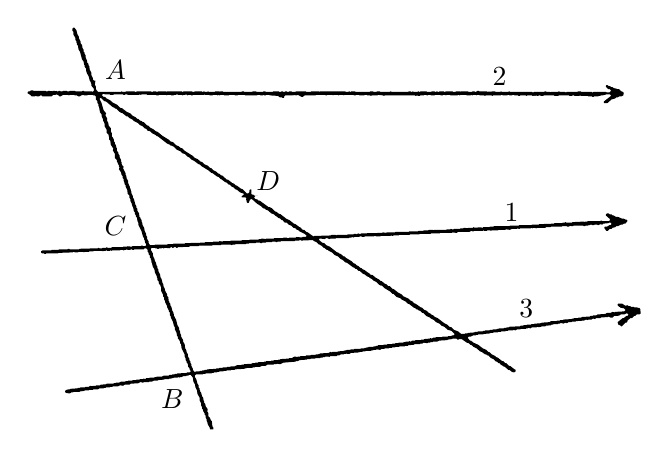
\begin{tikzpicture}[x=0.00651466cm,y=-0.00651466cm]
\fill[even odd rule] (13,148) -- (13,150) -- (18,153) -- (21,156) -- (27,156) -- (28,155) -- (30,155) -- (31,156) -- (35,156) -- (38,154) -- (40,154) -- (42,156) -- (59,156) -- (63,153) -- (67,153) -- (68,152) -- (72,153) -- (75,156) -- (77,156) -- (82,153) -- (92,153) -- (93,154) -- (95,153) -- (104,153) -- (105,154) -- (109,154) -- (112,156) -- (115,156) -- (117,154) -- (119,154) -- (120,153) -- (122,153) -- (123,154) -- (129,154) -- (130,153) -- (140,153) -- (141,154) -- (144,154) -- (146,156) -- (146,162) -- (148,164) -- (149,166) -- (149,169) -- (151,171) -- (151,175) -- (152,176) -- (154,187) -- (157,191) -- (157,194) -- (160,201) -- (160,204) -- (162,206) -- (162,208) -- (163,209) -- (163,214) -- (167,221) -- (167,227) -- (171,231) -- (171,234) -- (172,235) -- (172,240) -- (174,242) -- (175,250) -- (180,258) -- (179,261) -- (183,268) -- (183,276) -- (187,280) -- (187,283) -- (189,286) -- (189,288) -- (191,290) -- (191,293) -- (192,294) -- (191,298) -- (195,304) -- (196,309) -- (198,311) -- (198,315) -- (200,317) -- (200,321) -- (201,322) -- (202,327) -- (204,329) -- (204,332) -- (207,338) -- (208,346) -- (211,349) -- (211,353) -- (213,356) -- (213,359) -- (216,365) -- (216,367) -- (219,374) -- (220,380) -- (222,382) -- (222,385) -- (224,388) -- (224,390) -- (226,392) -- (227,399) -- (229,403) -- (229,407) -- (235,419) -- (238,430) -- (240,432) -- (240,435) -- (241,436) -- (242,441) -- (244,444) -- (244,446) -- (242,448) -- (238,448) -- (237,447) -- (234,447) -- (233,448) -- (217,448) -- (216,449) -- (208,448) -- (207,449) -- (199,449) -- (198,450) -- (177,450) -- (176,451) -- (169,451) -- (167,450) -- (166,451) -- (159,451) -- (158,452) -- (153,452) -- (151,451) -- (150,452) -- (114,453) -- (113,454) -- (95,454) -- (94,453) -- (92,453) -- (91,454) -- (74,454) -- (73,455) -- (60,455) -- (59,456) -- (42,456) -- (39,458) -- (39,460) -- (41,462) -- (45,462) -- (46,463) -- (48,463) -- (49,462) -- (72,462) -- (73,461) -- (101,460) -- (102,459) -- (104,459) -- (105,460) -- (111,460) -- (112,459) -- (121,459) -- (123,460) -- (124,459) -- (132,459) -- (133,458) -- (141,458) -- (142,457) -- (158,457) -- (160,458) -- (161,457) -- (165,457) -- (166,456) -- (168,457) -- (173,457) -- (174,456) -- (177,457) -- (178,456) -- (193,456) -- (194,455) -- (198,455) -- (199,456) -- (201,456) -- (202,455) -- (205,455) -- (206,454) -- (208,455) -- (213,455) -- (214,454) -- (216,454) -- (217,455) -- (220,455) -- (221,454) -- (239,454) -- (241,452) -- (244,452) -- (247,455) -- (247,459) -- (249,461) -- (249,464) -- (251,466) -- (251,470) -- (253,472) -- (253,474) -- (254,475) -- (254,479) -- (255,480) -- (257,488) -- (260,493) -- (261,499) -- (265,507) -- (265,509) -- (266,510) -- (266,514) -- (268,516) -- (269,521) -- (272,525) -- (272,527) -- (273,528) -- (273,535) -- (277,543) -- (277,546) -- (279,548) -- (279,552) -- (281,555) -- (281,557) -- (285,565) -- (285,567) -- (288,573) -- (288,575) -- (290,577) -- (290,582) -- (292,585) -- (292,587) -- (296,595) -- (298,603) -- (300,606) -- (300,610) -- (303,616) -- (304,622) -- (306,625) -- (306,628) -- (308,630) -- (310,634) -- (310,637) -- (312,639) -- (313,647) -- (319,659) -- (319,663) -- (321,667) -- (321,670) -- (323,673) -- (323,675) -- (325,677) -- (326,683) -- (328,685) -- (329,689) -- (331,691) -- (331,692) -- (329,694) -- (324,694) -- (323,695) -- (305,696) -- (304,697) -- (300,697) -- (299,698) -- (295,698) -- (294,699) -- (289,699) -- (288,700) -- (279,700) -- (275,702) -- (265,702) -- (264,703) -- (261,703) -- (260,704) -- (251,704) -- (250,705) -- (244,705) -- (242,707) -- (239,706) -- (238,707) -- (232,707) -- (231,708) -- (225,708) -- (224,709) -- (218,709) -- (217,710) -- (209,710) -- (208,711) -- (204,711) -- (203,712) -- (195,712) -- (191,714) -- (185,714) -- (184,715) -- (181,715) -- (180,716) -- (167,716) -- (166,717) -- (155,718) -- (154,719) -- (147,719) -- (146,720) -- (140,720) -- (139,721) -- (135,720) -- (132,722) -- (126,722) -- (125,723) -- (116,723) -- (115,724) -- (111,724) -- (110,725) -- (96,726) -- (95,727) -- (91,727) -- (90,728) -- (88,728) -- (86,730) -- (86,732) -- (88,734) -- (95,735) -- (98,733) -- (101,733) -- (102,732) -- (114,732) -- (115,731) -- (123,730) -- (124,729) -- (132,729) -- (133,728) -- (140,728) -- (141,727) -- (150,727) -- (153,725) -- (161,725) -- (162,724) -- (165,724) -- (166,723) -- (173,723) -- (174,722) -- (178,722) -- (179,721) -- (189,721) -- (193,719) -- (199,720) -- (202,718) -- (211,718) -- (214,716) -- (229,715) -- (232,713) -- (235,713) -- (236,714) -- (238,714) -- (239,713) -- (249,713) -- (250,712) -- (255,712) -- (259,710) -- (266,710) -- (267,709) -- (279,708) -- (280,707) -- (288,707) -- (289,706) -- (293,706) -- (294,705) -- (297,705) -- (298,704) -- (305,704) -- (306,703) -- (309,704) -- (310,703) -- (313,703) -- (317,701) -- (322,701) -- (323,700) -- (326,700) -- (327,699) -- (331,699) -- (335,704) -- (336,712) -- (339,717) -- (340,723) -- (343,729) -- (344,736) -- (348,743) -- (348,748) -- (351,754) -- (351,758) -- (353,762) -- (353,765) -- (355,767) -- (355,769) -- (358,774) -- (358,776) -- (360,778) -- (360,782) -- (362,786) -- (362,789) -- (363,790) -- (364,795) -- (368,802) -- (368,804) -- (369,805) -- (374,805) -- (375,804) -- (375,802) -- (373,799) -- (372,789) -- (370,787) -- (368,782) -- (365,779) -- (365,773) -- (363,770) -- (364,766) -- (360,760) -- (359,755) -- (357,753) -- (357,750) -- (356,749) -- (355,743) -- (353,741) -- (351,733) -- (349,731) -- (349,729) -- (348,728) -- (348,725) -- (346,723) -- (346,719) -- (344,716) -- (342,708) -- (339,703) -- (339,700) -- (341,698) -- (354,698) -- (355,697) -- (359,697) -- (360,696) -- (371,696) -- (372,695) -- (375,695) -- (376,694) -- (382,694) -- (383,693) -- (386,693) -- (387,692) -- (394,692) -- (395,691) -- (400,691) -- (401,690) -- (409,690) -- (410,689) -- (416,689) -- (417,688) -- (435,687) -- (436,686) -- (439,686) -- (440,685) -- (451,685) -- (452,684) -- (456,684) -- (457,683) -- (466,683) -- (470,681) -- (477,681) -- (480,679) -- (492,679) -- (493,678) -- (498,678) -- (499,677) -- (505,678) -- (511,675) -- (535,673) -- (536,672) -- (539,672) -- (543,670) -- (557,669) -- (558,668) -- (564,668) -- (565,667) -- (573,667) -- (574,666) -- (583,666) -- (584,665) -- (588,665) -- (589,664) -- (592,664) -- (593,663) -- (599,663) -- (601,664) -- (603,662) -- (615,662) -- (616,661) -- (620,661) -- (623,659) -- (629,659) -- (630,658) -- (633,658) -- (634,657) -- (636,658) -- (640,658) -- (643,656) -- (659,655) -- (660,654) -- (665,654) -- (666,653) -- (671,653) -- (672,652) -- (682,652) -- (683,651) -- (686,651) -- (687,650) -- (692,650) -- (693,649) -- (700,650) -- (703,648) -- (708,648) -- (709,647) -- (717,647) -- (718,646) -- (723,646) -- (724,645) -- (729,645) -- (730,644) -- (737,644) -- (738,643) -- (748,643) -- (749,642) -- (754,642) -- (755,641) -- (766,640) -- (767,639) -- (777,639) -- (778,638) -- (782,638) -- (785,636) -- (792,637) -- (793,636) -- (797,636) -- (798,635) -- (802,635) -- (803,634) -- (811,634) -- (815,632) -- (831,631) -- (832,630) -- (840,629) -- (841,628) -- (849,628) -- (851,630) -- (853,630) -- (854,629) -- (859,629) -- (869,636) -- (873,637) -- (876,640) -- (879,641) -- (882,644) -- (888,647) -- (895,653) -- (898,654) -- (905,659) -- (907,659) -- (909,661) -- (911,661) -- (916,666) -- (921,668) -- (926,673) -- (928,673) -- (931,676) -- (933,676) -- (936,680) -- (938,680) -- (940,682) -- (943,683) -- (950,689) -- (952,689) -- (957,693) -- (961,694) -- (964,692) -- (964,689) -- (963,688) -- (962,688) -- (953,681) -- (951,681) -- (946,676) -- (944,676) -- (940,672) -- (938,672) -- (929,665) -- (926,664) -- (924,662) -- (918,659) -- (914,655) -- (911,654) -- (907,650) -- (900,647) -- (891,640) -- (882,636) -- (877,632) -- (875,632) -- (871,627) -- (871,626) -- (873,624) -- (877,624) -- (881,622) -- (886,622) -- (887,621) -- (890,621) -- (891,620) -- (901,620) -- (902,619) -- (914,618) -- (915,617) -- (920,617) -- (921,616) -- (929,616) -- (930,615) -- (935,615) -- (936,614) -- (944,614) -- (945,613) -- (949,613) -- (950,612) -- (959,612) -- (960,611) -- (964,612) -- (967,610) -- (973,610) -- (974,609) -- (984,609) -- (985,608) -- (988,608) -- (989,607) -- (993,608) -- (996,606) -- (1005,606) -- (1006,605) -- (1010,606) -- (1011,605) -- (1014,605) -- (1015,604) -- (1022,604) -- (1023,603) -- (1033,602) -- (1034,601) -- (1037,601) -- (1038,600) -- (1046,600) -- (1047,599) -- (1050,599) -- (1051,598) -- (1055,598) -- (1057,599) -- (1061,597) -- (1064,598) -- (1067,596) -- (1073,596) -- (1074,595) -- (1081,595) -- (1082,594) -- (1097,593) -- (1101,591) -- (1105,592) -- (1106,591) -- (1112,591) -- (1115,589) -- (1119,590) -- (1121,588) -- (1129,588) -- (1130,587) -- (1144,586) -- (1145,585) -- (1149,587) -- (1153,587) -- (1156,584) -- (1164,584) -- (1165,583) -- (1167,583) -- (1169,581) -- (1176,581) -- (1180,579) -- (1182,579) -- (1184,581) -- (1184,582) -- (1182,584) -- (1180,584) -- (1175,588) -- (1173,588) -- (1163,596) -- (1164,600) -- (1166,602) -- (1168,602) -- (1170,604) -- (1171,604) -- (1178,597) -- (1180,597) -- (1182,595) -- (1182,593) -- (1188,588) -- (1191,588) -- (1195,584) -- (1197,584) -- (1200,581) -- (1205,581) -- (1208,579) -- (1207,570) -- (1205,568) -- (1202,568) -- (1201,567) -- (1195,567) -- (1194,566) -- (1189,566) -- (1188,565) -- (1185,565) -- (1182,563) -- (1178,564) -- (1172,560) -- (1164,560) -- (1163,561) -- (1163,563) -- (1166,566) -- (1167,566) -- (1169,568) -- (1175,569) -- (1178,572) -- (1178,573) -- (1176,575) -- (1158,576) -- (1157,577) -- (1153,576) -- (1149,578) -- (1142,578) -- (1139,580) -- (1124,581) -- (1121,583) -- (1115,583) -- (1114,584) -- (1110,584) -- (1109,585) -- (1093,586) -- (1092,587) -- (1087,587) -- (1086,588) -- (1078,588) -- (1077,589) -- (1074,589) -- (1073,590) -- (1057,591) -- (1056,592) -- (1051,592) -- (1050,593) -- (1045,593) -- (1044,594) -- (1033,594) -- (1030,596) -- (1015,597) -- (1014,598) -- (1001,599) -- (1000,600) -- (995,600) -- (994,601) -- (986,601) -- (985,602) -- (980,602) -- (979,603) -- (974,603) -- (973,604) -- (952,605) -- (951,606) -- (947,606) -- (946,607) -- (942,607) -- (941,608) -- (932,608) -- (931,609) -- (928,609) -- (927,610) -- (920,610) -- (919,611) -- (914,611) -- (913,612) -- (905,612) -- (904,613) -- (901,613) -- (900,614) -- (891,614) -- (890,615) -- (885,615) -- (884,616) -- (871,617) -- (870,618) -- (866,618) -- (865,619) -- (858,619) -- (852,614) -- (844,611) -- (839,606) -- (835,605) -- (831,601) -- (825,598) -- (812,588) -- (807,586) -- (804,583) -- (801,582) -- (799,580) -- (795,578) -- (791,574) -- (786,572) -- (782,568) -- (779,567) -- (769,560) -- (766,559) -- (762,555) -- (759,554) -- (755,550) -- (746,546) -- (742,542) -- (736,539) -- (727,532) -- (724,531) -- (719,526) -- (716,526) -- (712,522) -- (709,521) -- (703,516) -- (701,516) -- (698,513) -- (691,509) -- (685,504) -- (682,504) -- (678,500) -- (677,500) -- (669,494) -- (666,493) -- (664,491) -- (661,490) -- (658,487) -- (654,485) -- (651,482) -- (648,481) -- (644,477) -- (634,471) -- (631,468) -- (629,468) -- (623,463) -- (620,462) -- (618,460) -- (616,460) -- (602,449) -- (595,446) -- (591,442) -- (587,441) -- (581,436) -- (581,434) -- (582,433) -- (592,434) -- (595,432) -- (597,432) -- (598,433) -- (602,434) -- (603,433) -- (613,433) -- (614,432) -- (639,432) -- (640,431) -- (644,431) -- (645,430) -- (649,431) -- (650,430) -- (659,430) -- (660,429) -- (664,429) -- (665,430) -- (669,430) -- (670,429) -- (688,429) -- (689,428) -- (691,428) -- (692,429) -- (700,429) -- (701,428) -- (720,428) -- (721,427) -- (725,428) -- (726,427) -- (736,427) -- (737,426) -- (757,426) -- (758,425) -- (776,425) -- (777,424) -- (798,424) -- (799,423) -- (816,423) -- (817,422) -- (840,422) -- (841,421) -- (849,422) -- (852,420) -- (874,420) -- (878,418) -- (880,419) -- (882,419) -- (883,418) -- (900,418) -- (901,417) -- (903,418) -- (908,418) -- (909,417) -- (914,417) -- (916,418) -- (917,417) -- (930,417) -- (931,416) -- (944,416) -- (945,415) -- (953,416) -- (957,414) -- (967,414) -- (968,413) -- (970,414) -- (972,414) -- (973,413) -- (994,413) -- (995,412) -- (997,413) -- (999,412) -- (1005,413) -- (1006,412) -- (1022,412) -- (1023,411) -- (1032,411) -- (1033,410) -- (1054,410) -- (1055,409) -- (1064,409) -- (1065,410) -- (1067,410) -- (1071,408) -- (1073,409) -- (1076,409) -- (1077,408) -- (1096,408) -- (1097,409) -- (1099,409) -- (1100,408) -- (1105,408) -- (1106,407) -- (1109,407) -- (1110,406) -- (1112,406) -- (1113,407) -- (1117,407) -- (1118,406) -- (1123,406) -- (1125,407) -- (1129,405) -- (1133,406) -- (1135,404) -- (1145,403) -- (1146,402) -- (1149,402) -- (1151,404) -- (1151,405) -- (1149,407) -- (1147,407) -- (1142,410) -- (1138,410) -- (1137,411) -- (1137,413) -- (1139,415) -- (1139,416) -- (1141,418) -- (1144,418) -- (1148,414) -- (1151,414) -- (1153,412) -- (1158,411) -- (1160,409) -- (1163,409) -- (1169,406) -- (1172,406) -- (1175,404) -- (1178,404) -- (1182,399) -- (1182,398) -- (1180,396) -- (1178,396) -- (1174,394) -- (1171,394) -- (1164,391) -- (1160,391) -- (1155,388) -- (1153,388) -- (1151,386) -- (1148,386) -- (1145,384) -- (1142,384) -- (1140,386) -- (1140,388) -- (1148,395) -- (1148,397) -- (1146,399) -- (1133,399) -- (1132,398) -- (1130,398) -- (1129,399) -- (1105,399) -- (1104,400) -- (1100,400) -- (1099,401) -- (1097,400) -- (1075,401) -- (1074,402) -- (1063,402) -- (1061,401) -- (1060,402) -- (1056,402) -- (1055,403) -- (1040,403) -- (1039,404) -- (1010,405) -- (1009,406) -- (996,406) -- (995,407) -- (971,407) -- (970,408) -- (953,408) -- (952,409) -- (922,409) -- (921,410) -- (914,410) -- (913,411) -- (901,411) -- (900,412) -- (898,412) -- (897,411) -- (884,412) -- (882,411) -- (881,412) -- (872,412) -- (871,413) -- (863,412) -- (862,413) -- (857,413) -- (856,414) -- (844,414) -- (843,415) -- (840,415) -- (838,414) -- (837,415) -- (830,415) -- (829,416) -- (805,416) -- (804,417) -- (802,416) -- (795,416) -- (794,417) -- (785,417) -- (784,418) -- (775,418) -- (774,419) -- (757,419) -- (756,420) -- (730,420) -- (729,421) -- (713,421) -- (712,422) -- (705,421) -- (704,422) -- (663,423) -- (662,424) -- (659,424) -- (657,423) -- (655,425) -- (653,424) -- (649,424) -- (648,425) -- (637,425) -- (636,426) -- (616,426) -- (615,427) -- (613,426) -- (605,426) -- (604,427) -- (572,428) -- (570,429) -- (559,421) -- (556,420) -- (552,416) -- (549,416) -- (544,411) -- (543,411) -- (535,405) -- (532,404) -- (523,397) -- (518,395) -- (505,385) -- (503,385) -- (498,381) -- (495,380) -- (489,374) -- (485,372) -- (483,372) -- (465,359) -- (463,359) -- (461,357) -- (457,356) -- (455,354) -- (455,352) -- (457,350) -- (461,350) -- (456,350) -- (454,348) -- (450,347) -- (449,346) -- (449,338) -- (448,337) -- (446,338) -- (445,340) -- (445,343) -- (443,345) -- (440,345) -- (432,337) -- (429,336) -- (421,330) -- (418,329) -- (415,326) -- (412,325) -- (403,318) -- (401,318) -- (392,310) -- (390,310) -- (387,307) -- (384,306) -- (381,303) -- (375,300) -- (371,296) -- (368,295) -- (364,291) -- (357,288) -- (353,284) -- (350,283) -- (344,278) -- (339,276) -- (335,272) -- (319,262) -- (314,257) -- (312,257) -- (307,253) -- (302,251) -- (296,245) -- (292,244) -- (289,241) -- (276,233) -- (266,225) -- (263,224) -- (258,220) -- (252,217) -- (248,213) -- (245,212) -- (239,206) -- (237,206) -- (235,204) -- (232,203) -- (229,200) -- (227,200) -- (224,197) -- (218,194) -- (213,189) -- (206,186) -- (197,179) -- (193,178) -- (187,172) -- (179,168) -- (173,163) -- (167,160) -- (164,157) -- (161,157) -- (158,154) -- (158,153) -- (160,151) -- (162,151) -- (163,152) -- (173,152) -- (174,153) -- (180,153) -- (181,152) -- (199,152) -- (200,153) -- (202,153) -- (203,152) -- (207,152) -- (208,153) -- (230,153) -- (231,152) -- (234,153) -- (235,152) -- (245,152) -- (246,153) -- (263,153) -- (264,154) -- (268,154) -- (269,153) -- (283,153) -- (284,154) -- (286,153) -- (292,153) -- (293,154) -- (297,154) -- (298,153) -- (302,153) -- (303,152) -- (305,152) -- (306,153) -- (314,153) -- (315,154) -- (317,153) -- (320,153) -- (321,152) -- (322,152) -- (324,154) -- (326,153) -- (331,153) -- (332,154) -- (334,154) -- (335,153) -- (356,153) -- (357,152) -- (359,153) -- (367,153) -- (368,154) -- (373,154) -- (374,153) -- (382,153) -- (383,154) -- (385,153) -- (387,154) -- (389,153) -- (395,153) -- (396,154) -- (405,154) -- (406,153) -- (416,153) -- (417,154) -- (422,154) -- (423,153) -- (436,153) -- (437,154) -- (460,154) -- (461,153) -- (466,153) -- (467,154) -- (471,154) -- (473,153) -- (474,154) -- (477,154) -- (478,153) -- (484,153) -- (485,154) -- (501,155) -- (505,158) -- (509,158) -- (510,159) -- (512,159) -- (513,158) -- (513,156) -- (515,154) -- (529,154) -- (530,153) -- (532,154) -- (534,153) -- (536,154) -- (540,153) -- (547,157) -- (549,157) -- (553,154) -- (574,154) -- (575,153) -- (593,153) -- (594,154) -- (596,154) -- (597,153) -- (607,153) -- (608,154) -- (610,153) -- (618,153) -- (619,154) -- (621,153) -- (628,153) -- (629,154) -- (631,153) -- (648,153) -- (649,154) -- (652,154) -- (653,153) -- (659,153) -- (660,154) -- (669,154) -- (670,153) -- (674,153) -- (675,154) -- (681,154) -- (682,155) -- (684,154) -- (695,154) -- (696,153) -- (706,154) -- (707,155) -- (709,154) -- (768,154) -- (769,155) -- (773,154) -- (774,155) -- (777,155) -- (778,154) -- (785,154) -- (786,153) -- (790,153) -- (791,154) -- (793,154) -- (794,153) -- (798,153) -- (799,154) -- (806,154) -- (807,153) -- (817,153) -- (818,154) -- (822,154) -- (823,153) -- (827,153) -- (828,154) -- (830,153) -- (836,153) -- (837,154) -- (851,154) -- (852,153) -- (854,153) -- (855,154) -- (857,153) -- (868,153) -- (869,154) -- (876,154) -- (878,153) -- (880,154) -- (881,153) -- (886,153) -- (888,154) -- (889,153) -- (893,153) -- (894,154) -- (903,154) -- (904,155) -- (906,154) -- (917,154) -- (919,155) -- (920,154) -- (935,154) -- (936,153) -- (938,153) -- (939,154) -- (948,154) -- (949,153) -- (951,153) -- (952,154) -- (957,154) -- (958,153) -- (961,153) -- (962,154) -- (969,154) -- (970,155) -- (972,155) -- (973,154) -- (984,154) -- (985,155) -- (987,154) -- (996,154) -- (997,155) -- (999,155) -- (1000,154) -- (1002,155) -- (1004,154) -- (1006,155) -- (1008,155) -- (1009,154) -- (1012,154) -- (1013,155) -- (1018,155) -- (1019,154) -- (1039,154) -- (1040,155) -- (1047,155) -- (1048,154) -- (1068,154) -- (1069,155) -- (1074,155) -- (1075,154) -- (1078,154) -- (1079,155) -- (1088,155) -- (1090,154) -- (1091,155) -- (1105,155) -- (1106,156) -- (1113,156) -- (1114,157) -- (1116,157) -- (1117,156) -- (1125,156) -- (1126,155) -- (1129,155) -- (1130,154) -- (1135,154) -- (1136,153) -- (1139,153) -- (1140,152) -- (1148,152) -- (1150,154) -- (1150,155) -- (1136,166) -- (1136,168) -- (1137,169) -- (1143,169) -- (1151,162) -- (1158,160) -- (1160,158) -- (1163,158) -- (1166,156) -- (1170,156) -- (1174,154) -- (1175,149) -- (1173,147) -- (1170,146) -- (1166,142) -- (1162,142) -- (1161,141) -- (1156,140) -- (1153,138) -- (1151,138) -- (1148,136) -- (1146,136) -- (1143,134) -- (1141,134) -- (1140,135) -- (1140,137) -- (1145,142) -- (1148,142) -- (1150,144) -- (1150,145) -- (1147,148) -- (1141,148) -- (1140,147) -- (1116,147) -- (1115,148) -- (1113,148) -- (1112,147) -- (1092,147) -- (1091,146) -- (1086,146) -- (1085,147) -- (1064,147) -- (1063,148) -- (1061,148) -- (1060,147) -- (1050,147) -- (1049,146) -- (1047,147) -- (1033,147) -- (1032,148) -- (1030,147) -- (1024,147) -- (1023,146) -- (1021,146) -- (1020,147) -- (1000,147) -- (999,148) -- (997,148) -- (996,147) -- (953,147) -- (952,146) -- (950,147) -- (937,147) -- (936,146) -- (934,147) -- (925,147) -- (924,146) -- (909,147) -- (908,146) -- (893,146) -- (892,145) -- (890,145) -- (887,147) -- (885,147) -- (884,146) -- (880,146) -- (879,147) -- (872,147) -- (871,146) -- (858,146) -- (857,147) -- (855,146) -- (848,146) -- (847,147) -- (842,147) -- (841,146) -- (828,146) -- (827,147) -- (825,147) -- (824,146) -- (816,146) -- (815,147) -- (812,147) -- (811,146) -- (809,147) -- (807,147) -- (806,146) -- (801,146) -- (800,147) -- (791,147) -- (790,146) -- (779,146) -- (778,147) -- (776,147) -- (775,146) -- (773,147) -- (765,147) -- (764,146) -- (762,147) -- (760,147) -- (759,146) -- (756,146) -- (755,147) -- (722,147) -- (721,146) -- (719,147) -- (700,147) -- (699,146) -- (694,146) -- (693,147) -- (687,147) -- (686,146) -- (681,146) -- (680,147) -- (652,147) -- (651,146) -- (644,146) -- (643,147) -- (641,147) -- (640,146) -- (638,147) -- (633,147) -- (632,146) -- (583,146) -- (582,147) -- (580,146) -- (566,146) -- (565,147) -- (556,147) -- (555,146) -- (536,146) -- (535,147) -- (528,147) -- (527,146) -- (523,146) -- (522,147) -- (519,147) -- (518,146) -- (515,146) -- (514,147) -- (511,147) -- (510,146) -- (508,146) -- (507,147) -- (503,147) -- (502,146) -- (492,146) -- (491,147) -- (477,147) -- (476,146) -- (473,146) -- (472,147) -- (459,147) -- (458,146) -- (452,146) -- (451,147) -- (435,147) -- (434,146) -- (431,146) -- (430,147) -- (394,147) -- (393,146) -- (389,146) -- (388,147) -- (386,146) -- (379,146) -- (378,147) -- (366,147) -- (365,146) -- (363,147) -- (358,147) -- (357,146) -- (355,147) -- (353,147) -- (352,146) -- (339,146) -- (338,147) -- (334,147) -- (333,146) -- (317,146) -- (316,147) -- (314,147) -- (313,146) -- (285,146) -- (284,147) -- (282,146) -- (267,146) -- (266,147) -- (264,147) -- (263,146) -- (258,146) -- (257,147) -- (254,147) -- (253,146) -- (226,146) -- (225,147) -- (222,147) -- (221,146) -- (205,146) -- (204,147) -- (198,147) -- (196,146) -- (195,147) -- (150,147) -- (146,142) -- (146,137) -- (144,133) -- (145,125) -- (142,125) -- (140,123) -- (140,120) -- (137,114) -- (137,110) -- (134,104) -- (133,97) -- (132,96) -- (131,92) -- (129,90) -- (129,87) -- (126,80) -- (126,76) -- (124,73) -- (124,71) -- (122,69) -- (122,65) -- (120,62) -- (119,56) -- (116,52) -- (116,49) -- (113,43) -- (113,40) -- (110,35) -- (108,27) -- (104,22) -- (102,22) -- (100,24) -- (100,28) -- (102,30) -- (102,35) -- (106,42) -- (106,46) -- (108,48) -- (108,51) -- (109,52) -- (109,55) -- (111,57) -- (112,64) -- (115,69) -- (119,84) -- (122,88) -- (123,94) -- (124,95) -- (124,98) -- (127,102) -- (127,107) -- (128,108) -- (128,110) -- (132,117) -- (134,125) -- (136,128) -- (136,130) -- (137,131) -- (137,135) -- (142,141) -- (142,145) -- (140,147) -- (139,147) -- (138,146) -- (123,146) -- (122,145) -- (120,145) -- (119,146) -- (106,146) -- (105,145) -- (95,145) -- (94,146) -- (90,146) -- (89,145) -- (82,145) -- (81,146) -- (77,146) -- (76,145) -- (74,145) -- (73,146) -- (70,146) -- (69,145) -- (67,146) -- (65,145) -- (62,145) -- (61,146) -- (53,145) -- (52,146) -- (49,146) -- (48,145) -- (24,145) -- (23,144) -- (20,144) -- (17,146) -- (15,146) -- cycle
(253,453) -- (255,451) -- (261,451) -- (262,452) -- (265,452) -- (266,453) -- (268,453) -- (269,452) -- (274,452) -- (275,451) -- (277,452) -- (279,452) -- (280,451) -- (289,452) -- (292,450) -- (294,450) -- (295,451) -- (297,451) -- (298,450) -- (302,450) -- (303,451) -- (305,451) -- (306,450) -- (328,449) -- (329,448) -- (346,448) -- (347,447) -- (372,447) -- (373,446) -- (389,446) -- (390,445) -- (409,445) -- (411,446) -- (412,445) -- (417,445) -- (418,444) -- (438,444) -- (439,443) -- (444,443) -- (445,442) -- (457,442) -- (458,441) -- (466,441) -- (467,442) -- (469,442) -- (470,441) -- (477,441) -- (478,440) -- (489,440) -- (490,439) -- (496,439) -- (497,440) -- (499,440) -- (500,439) -- (506,439) -- (507,438) -- (533,438) -- (534,437) -- (542,437) -- (543,436) -- (545,436) -- (546,437) -- (569,436) -- (571,438) -- (576,440) -- (581,445) -- (583,445) -- (585,447) -- (586,447) -- (590,451) -- (591,451) -- (596,455) -- (598,455) -- (600,457) -- (606,460) -- (611,465) -- (618,468) -- (623,473) -- (626,474) -- (633,480) -- (635,480) -- (647,489) -- (650,490) -- (652,492) -- (654,492) -- (658,496) -- (660,496) -- (667,502) -- (670,503) -- (675,507) -- (678,508) -- (680,510) -- (684,512) -- (687,515) -- (693,518) -- (698,523) -- (702,525) -- (704,525) -- (709,530) -- (719,536) -- (724,541) -- (726,541) -- (732,547) -- (739,549) -- (742,552) -- (750,556) -- (754,560) -- (757,561) -- (766,568) -- (768,568) -- (771,571) -- (773,571) -- (775,573) -- (778,574) -- (782,578) -- (784,578) -- (790,584) -- (797,587) -- (799,589) -- (805,592) -- (809,596) -- (816,599) -- (820,603) -- (825,605) -- (832,611) -- (839,613) -- (845,619) -- (845,620) -- (843,622) -- (840,622) -- (839,623) -- (833,623) -- (832,624) -- (822,624) -- (821,625) -- (809,625) -- (808,626) -- (804,626) -- (801,628) -- (798,627) -- (797,628) -- (786,629) -- (785,630) -- (780,630) -- (779,631) -- (769,631) -- (768,632) -- (762,632) -- (760,634) -- (757,633) -- (756,634) -- (750,634) -- (749,635) -- (746,635) -- (745,636) -- (736,636) -- (735,637) -- (730,637) -- (729,638) -- (724,638) -- (723,639) -- (714,639) -- (713,640) -- (707,640) -- (706,641) -- (696,641) -- (695,642) -- (692,642) -- (691,643) -- (688,643) -- (687,644) -- (678,644) -- (677,645) -- (674,645) -- (673,646) -- (670,646) -- (669,647) -- (663,647) -- (662,648) -- (650,648) -- (649,649) -- (643,649) -- (642,650) -- (635,650) -- (634,651) -- (631,651) -- (630,652) -- (618,653) -- (617,654) -- (607,654) -- (606,655) -- (603,654) -- (600,656) -- (583,657) -- (582,658) -- (580,658) -- (579,659) -- (575,659) -- (574,660) -- (565,660) -- (564,661) -- (556,661) -- (555,662) -- (545,662) -- (544,663) -- (540,663) -- (539,664) -- (533,663) -- (528,666) -- (523,666) -- (522,667) -- (506,668) -- (505,669) -- (502,669) -- (501,670) -- (493,670) -- (492,671) -- (488,671) -- (487,672) -- (478,672) -- (477,673) -- (474,673) -- (473,674) -- (463,674) -- (462,675) -- (457,675) -- (456,676) -- (451,676) -- (450,677) -- (435,678) -- (434,679) -- (430,679) -- (429,680) -- (421,680) -- (417,682) -- (409,682) -- (408,683) -- (402,683) -- (401,684) -- (394,684) -- (393,685) -- (387,685) -- (386,686) -- (381,686) -- (380,687) -- (363,688) -- (362,689) -- (358,689) -- (357,690) -- (354,690) -- (353,691) -- (349,691) -- (348,692) -- (341,692) -- (340,693) -- (338,693) -- (335,689) -- (335,687) -- (332,681) -- (332,678) -- (330,675) -- (330,672) -- (328,670) -- (328,667) -- (326,664) -- (325,658) -- (323,655) -- (322,650) -- (320,647) -- (319,639) -- (316,634) -- (316,631) -- (312,624) -- (312,621) -- (310,617) -- (310,614) -- (308,610) -- (308,607) -- (305,602) -- (302,590) -- (300,588) -- (300,586) -- (298,584) -- (298,580) -- (297,579) -- (297,577) -- (295,574) -- (293,566) -- (291,563) -- (291,560) -- (289,558) -- (289,556) -- (288,555) -- (287,547) -- (285,545) -- (285,542) -- (281,535) -- (280,530) -- (278,527) -- (277,521) -- (276,520) -- (274,512) -- (272,509) -- (271,503) -- (268,497) -- (268,494) -- (266,491) -- (266,488) -- (264,485) -- (263,480) -- (261,477) -- (260,472) -- (258,469) -- (258,467) -- (257,466) -- (257,462) -- (253,455) -- cycle
(153,161) -- (155,159) -- (156,159) -- (162,165) -- (166,166) -- (179,177) -- (182,178) -- (184,180) -- (186,180) -- (192,186) -- (193,186) -- (195,188) -- (197,188) -- (206,195) -- (208,195) -- (211,198) -- (217,201) -- (220,204) -- (228,208) -- (232,212) -- (237,214) -- (242,219) -- (244,219) -- (247,223) -- (252,224) -- (256,228) -- (262,231) -- (264,233) -- (267,234) -- (285,248) -- (290,250) -- (292,252) -- (294,252) -- (298,254) -- (304,260) -- (311,263) -- (315,267) -- (319,268) -- (324,273) -- (328,275) -- (332,279) -- (338,282) -- (346,288) -- (349,289) -- (352,292) -- (365,300) -- (371,305) -- (374,306) -- (382,312) -- (385,313) -- (389,317) -- (390,317) -- (398,323) -- (401,324) -- (405,328) -- (407,328) -- (411,332) -- (414,333) -- (418,337) -- (421,338) -- (427,343) -- (433,345) -- (434,346) -- (434,348) -- (432,349) -- (430,351) -- (430,352) -- (431,353) -- (438,353) -- (440,355) -- (439,356) -- (439,358) -- (440,359) -- (440,362) -- (442,364) -- (444,363) -- (446,358) -- (448,356) -- (450,356) -- (460,365) -- (468,370) -- (472,374) -- (474,374) -- (478,377) -- (481,378) -- (488,384) -- (493,386) -- (496,389) -- (497,389) -- (502,393) -- (505,394) -- (508,397) -- (510,397) -- (513,401) -- (515,402) -- (518,402) -- (522,406) -- (527,408) -- (531,412) -- (535,413) -- (538,416) -- (540,416) -- (543,419) -- (553,424) -- (557,428) -- (555,430) -- (549,430) -- (548,431) -- (537,430) -- (536,431) -- (523,431) -- (522,432) -- (519,432) -- (518,431) -- (512,431) -- (511,432) -- (494,432) -- (493,433) -- (478,433) -- (477,434) -- (469,433) -- (468,434) -- (464,434) -- (463,435) -- (446,435) -- (445,436) -- (431,436) -- (430,437) -- (409,437) -- (408,438) -- (394,438) -- (393,439) -- (387,438) -- (386,439) -- (375,439) -- (374,440) -- (359,440) -- (358,441) -- (320,442) -- (319,443) -- (297,443) -- (296,444) -- (286,444) -- (285,445) -- (261,445) -- (260,446) -- (252,446) -- (250,444) -- (249,442) -- (249,439) -- (246,434) -- (246,430) -- (244,427) -- (244,424) -- (241,418) -- (240,412) -- (237,407) -- (236,401) -- (235,400) -- (235,397) -- (233,395) -- (233,393) -- (231,391) -- (230,384) -- (227,379) -- (227,375) -- (225,373) -- (225,370) -- (223,367) -- (220,356) -- (218,353) -- (218,350) -- (215,344) -- (215,341) -- (214,340) -- (214,338) -- (213,337) -- (213,335) -- (212,334) -- (212,332) -- (209,325) -- (209,321) -- (206,316) -- (205,310) -- (204,309) -- (204,306) -- (199,296) -- (200,293) -- (198,291) -- (196,287) -- (196,284) -- (195,283) -- (195,280) -- (192,274) -- (192,271) -- (190,268) -- (190,266) -- (187,262) -- (187,257) -- (186,256) -- (185,251) -- (183,249) -- (183,246) -- (181,243) -- (181,240) -- (179,236) -- (177,234) -- (177,228) -- (175,224) -- (175,218) -- (171,213) -- (170,207) -- (168,204) -- (168,199) -- (165,194) -- (165,191) -- (166,189) -- (161,183) -- (157,169) -- cycle;
\node[inner sep=0pt] at (184,104) {$A$};
\node[inner sep=0pt] at (933,118) {$2$};
\node[inner sep=0pt] at (482,320) {$D$};
\node[inner sep=0pt] at (956,382) {$1$};
\node[inner sep=0pt] at (184,409) {$C$};
\node[inner sep=0pt] at (985,569) {$3$};
\node[inner sep=0pt] at (295,746) {$B$};
\end{tikzpicture}

\end{center}
\noindent Punkte auf $2$ und $3$ und $AB$ schneide die $1$ in $C$. Durch $A$ ziehe man eine beliebige Gerade $AD\mathinner{.\,.\,.}$ zwischen $2$ und $AB$, welche also $1$ schneiden wird; weiter fortgesetzt wird sie also auch $3$ schneiden; da diess von jeder $AD\mathinner{.\,.\,.}$ gilt, so ist $2$ mit $3$ parallel. 

Zweiter Fall, wenn $1$ ausserhalb $2$ und $3$ liegt. Es liege $2$ zwischen $1$

\begin{center}
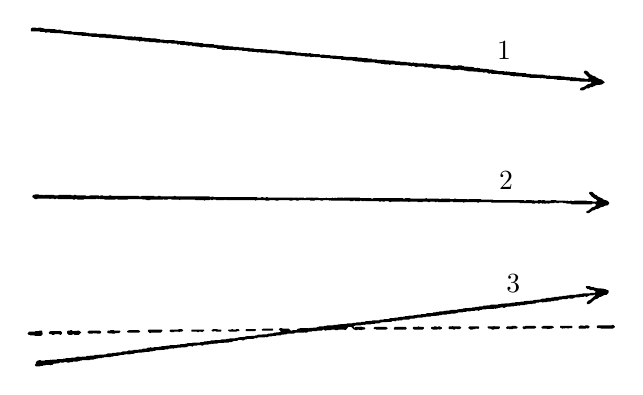
\begin{tikzpicture}[x=0.00656997cm,y=-0.00656997cm]
\fill[even odd rule] (58,600) -- (58,602) -- (60,604) -- (63,604) -- (64,605) -- (68,605) -- (69,604) -- (78,604) -- (79,605) -- (81,605) -- (83,603) -- (83,600) -- (81,598) -- (61,598) -- cycle
(133,599) -- (133,601) -- (136,603) -- (142,603) -- (143,602) -- (157,603) -- (159,600) -- (159,599) -- (156,597) -- (136,597) -- cycle
(46,604) -- (45,598) -- (44,597) -- (40,597) -- (39,598) -- (32,598) -- (31,599) -- (20,599) -- (17,602) -- (17,603) -- (19,605) -- (21,605) -- (22,606) -- (30,606) -- (31,607) -- (43,607) -- cycle
(209,598) -- (209,599) -- (211,601) -- (232,601) -- (234,599) -- (234,598) -- (231,596) -- (213,596) -- cycle
(171,601) -- (172,602) -- (185,603) -- (186,602) -- (193,602) -- (196,599) -- (196,598) -- (195,597) -- (184,597) -- (183,596) -- (177,596) -- (176,597) -- (172,597) -- (171,598) -- cycle
(93,599) -- (93,602) -- (96,605) -- (103,605) -- (104,604) -- (106,604) -- (107,605) -- (116,605) -- (120,601) -- (120,600) -- (116,597) -- (104,598) -- (102,596) -- (100,596) -- (99,597) -- (95,597) -- cycle
(333,596) -- (333,598) -- (334,599) -- (344,599) -- (345,600) -- (347,600) -- (348,599) -- (352,599) -- (354,600) -- (358,597) -- (357,595) -- (334,595) -- cycle
(249,597) -- (249,598) -- (253,602) -- (255,601) -- (274,601) -- (277,598) -- (277,596) -- (276,595) -- (251,595) -- cycle
(438,595) -- (438,597) -- (439,598) -- (456,598) -- (458,596) -- (457,594) -- (439,594) -- cycle
(404,596) -- (404,597) -- (407,599) -- (420,599) -- (421,598) -- (425,598) -- (426,597) -- (426,596) -- (424,594) -- (420,594) -- (419,595) -- (414,595) -- (413,594) -- (411,594) -- (410,595) -- (405,595) -- cycle
(372,596) -- (372,597) -- (375,599) -- (377,598) -- (380,598) -- (381,599) -- (390,599) -- (391,598) -- (391,596) -- (390,595) -- (384,595) -- (383,594) -- (376,594) -- cycle
(317,596) -- (314,594) -- (309,594) -- (308,595) -- (293,595) -- (291,597) -- (291,598) -- (294,600) -- (299,600) -- (300,599) -- (308,599) -- (310,600) -- (311,599) -- (315,599) -- (317,597) -- cycle
(469,595) -- (470,597) -- (490,597) -- (491,596) -- (491,594) -- (490,593) -- (472,593) -- cycle
(724,592) -- (724,594) -- (725,595) -- (747,595) -- (749,593) -- (749,592) -- (747,590) -- (726,590) -- cycle
(685,592) -- (686,594) -- (689,594) -- (690,595) -- (709,595) -- (712,593) -- (712,592) -- (709,590) -- (687,590) -- cycle
(868,591) -- (868,592) -- (872,595) -- (876,595) -- (877,594) -- (881,594) -- (882,593) -- (885,593) -- (887,594) -- (889,592) -- (889,590) -- (888,589) -- (870,589) -- cycle
(796,591) -- (796,593) -- (800,595) -- (808,595) -- (809,594) -- (813,595) -- (817,593) -- (817,591) -- (813,589) -- (810,589) -- (809,590) -- (807,590) -- (806,589) -- (802,589) -- (801,590) -- (797,590) -- cycle
(761,591) -- (761,593) -- (763,595) -- (780,595) -- (782,593) -- (782,591) -- (781,590) -- (774,590) -- (773,589) -- (771,589) -- (770,590) -- (762,590) -- cycle
(1045,589) -- (1045,591) -- (1049,593) -- (1051,593) -- (1052,592) -- (1054,593) -- (1056,592) -- (1061,593) -- (1062,592) -- (1068,592) -- (1069,591) -- (1069,589) -- (1068,588) -- (1046,588) -- cycle
(1009,590) -- (1009,591) -- (1011,593) -- (1019,593) -- (1020,594) -- (1029,593) -- (1033,591) -- (1033,590) -- (1030,588) -- (1013,588) -- cycle
(973,590) -- (973,592) -- (975,594) -- (978,594) -- (979,593) -- (996,593) -- (999,591) -- (999,590) -- (997,588) -- (978,588) -- (977,589) -- (974,589) -- cycle
(963,590) -- (959,588) -- (952,588) -- (951,589) -- (943,589) -- (941,591) -- (941,592) -- (943,594) -- (945,593) -- (947,594) -- (954,594) -- (955,593) -- (961,593) -- (963,591) -- cycle
(905,590) -- (905,591) -- (907,593) -- (910,593) -- (914,595) -- (917,595) -- (918,594) -- (926,594) -- (929,592) -- (929,590) -- (928,589) -- (919,589) -- (918,588) -- (916,589) -- (906,589) -- cycle
(830,590) -- (830,593) -- (831,594) -- (838,594) -- (839,595) -- (842,595) -- (844,593) -- (846,594) -- (851,594) -- (854,592) -- (854,591) -- (852,589) -- (839,589) -- (837,588) -- (836,589) -- (831,589) -- cycle
(1081,592) -- (1082,593) -- (1095,593) -- (1096,592) -- (1099,593) -- (1102,590) -- (1102,589) -- (1099,587) -- (1094,587) -- (1093,588) -- (1085,587) -- (1081,589) -- cycle
(1151,589) -- (1148,586) -- (1146,586) -- (1145,587) -- (1118,587) -- (1116,589) -- (1116,591) -- (1117,592) -- (1123,592) -- (1124,593) -- (1147,593) -- (1149,592) -- (1151,590) -- cycle
(1139,520) -- (1138,519) -- (1136,519) -- (1133,517) -- (1130,517) -- (1129,516) -- (1114,515) -- (1113,514) -- (1111,514) -- (1110,513) -- (1106,513) -- (1102,511) -- (1096,511) -- (1095,512) -- (1095,514) -- (1098,517) -- (1101,517) -- (1104,519) -- (1110,519) -- (1114,522) -- (1112,524) -- (1104,524) -- (1103,525) -- (1089,525) -- (1088,526) -- (1082,526) -- (1081,527) -- (1077,527) -- (1076,528) -- (1064,528) -- (1063,529) -- (1058,529) -- (1057,530) -- (1050,530) -- (1049,531) -- (1043,531) -- (1042,532) -- (1034,532) -- (1033,533) -- (1029,533) -- (1028,534) -- (1018,534) -- (1017,535) -- (1011,535) -- (1007,537) -- (994,538) -- (993,539) -- (976,540) -- (975,541) -- (969,541) -- (968,542) -- (959,542) -- (958,543) -- (952,543) -- (951,544) -- (932,545) -- (931,546) -- (926,546) -- (925,547) -- (911,547) -- (910,548) -- (897,549) -- (896,550) -- (889,550) -- (888,551) -- (882,551) -- (881,552) -- (876,552) -- (875,553) -- (858,554) -- (857,555) -- (847,556) -- (846,557) -- (834,557) -- (833,558) -- (821,559) -- (820,560) -- (812,560) -- (811,561) -- (806,561) -- (805,562) -- (800,562) -- (799,563) -- (789,563) -- (785,565) -- (777,565) -- (776,566) -- (769,566) -- (768,567) -- (763,567) -- (762,568) -- (753,568) -- (752,569) -- (746,569) -- (745,570) -- (733,571) -- (732,572) -- (726,572) -- (725,573) -- (717,573) -- (713,575) -- (705,575) -- (704,576) -- (697,576) -- (696,577) -- (683,577) -- (682,578) -- (669,579) -- (668,580) -- (662,580) -- (661,581) -- (652,581) -- (651,582) -- (645,582) -- (644,583) -- (634,583) -- (633,584) -- (616,585) -- (615,586) -- (608,586) -- (607,587) -- (595,587) -- (594,588) -- (590,588) -- (589,589) -- (580,589) -- (579,590) -- (576,590) -- (575,591) -- (561,592) -- (560,593) -- (558,592) -- (543,592) -- (542,593) -- (539,593) -- (536,596) -- (529,596) -- (528,597) -- (525,597) -- (521,593) -- (509,593) -- (508,592) -- (505,592) -- (502,594) -- (502,595) -- (506,598) -- (504,600) -- (493,601) -- (492,602) -- (481,603) -- (480,604) -- (461,605) -- (460,606) -- (457,606) -- (456,607) -- (438,608) -- (437,609) -- (424,610) -- (423,611) -- (419,611) -- (418,612) -- (407,612) -- (406,613) -- (401,613) -- (400,614) -- (391,614) -- (390,615) -- (371,616) -- (370,617) -- (358,618) -- (357,619) -- (351,619) -- (350,620) -- (336,620) -- (335,621) -- (326,621) -- (325,622) -- (322,622) -- (321,623) -- (312,623) -- (311,624) -- (306,624) -- (305,625) -- (292,625) -- (291,626) -- (285,626) -- (284,627) -- (276,627) -- (275,628) -- (271,628) -- (270,629) -- (261,629) -- (260,630) -- (256,630) -- (254,629) -- (253,630) -- (249,630) -- (246,632) -- (239,632) -- (238,633) -- (232,633) -- (231,634) -- (222,634) -- (221,635) -- (218,635) -- (217,636) -- (213,635) -- (209,637) -- (201,637) -- (197,639) -- (189,639) -- (188,640) -- (181,640) -- (180,641) -- (172,641) -- (168,643) -- (147,644) -- (146,645) -- (131,646) -- (130,647) -- (122,647) -- (121,648) -- (113,647) -- (109,649) -- (102,649) -- (101,650) -- (91,650) -- (90,651) -- (86,651) -- (85,652) -- (74,652) -- (73,653) -- (64,653) -- (63,654) -- (61,653) -- (59,654) -- (51,654) -- (50,655) -- (43,655) -- (42,654) -- (39,654) -- (38,655) -- (36,655) -- (33,658) -- (33,661) -- (31,663) -- (31,664) -- (33,666) -- (41,666) -- (42,665) -- (46,665) -- (47,664) -- (51,664) -- (52,663) -- (59,663) -- (61,664) -- (62,663) -- (65,663) -- (67,661) -- (77,660) -- (80,658) -- (82,659) -- (86,659) -- (87,658) -- (93,658) -- (94,659) -- (97,659) -- (98,658) -- (103,658) -- (106,656) -- (108,657) -- (113,657) -- (114,656) -- (117,656) -- (118,655) -- (121,655) -- (122,654) -- (137,654) -- (138,653) -- (144,653) -- (145,652) -- (148,652) -- (149,651) -- (152,651) -- (153,650) -- (160,650) -- (161,649) -- (164,649) -- (165,648) -- (177,648) -- (178,647) -- (182,647) -- (183,646) -- (191,646) -- (192,645) -- (195,645) -- (196,644) -- (203,644) -- (204,643) -- (207,643) -- (208,642) -- (210,643) -- (215,643) -- (216,642) -- (221,642) -- (225,640) -- (242,639) -- (243,638) -- (252,638) -- (253,637) -- (258,637) -- (259,636) -- (263,636) -- (264,635) -- (281,634) -- (282,633) -- (288,633) -- (289,632) -- (294,632) -- (295,631) -- (299,632) -- (300,631) -- (305,631) -- (306,630) -- (324,629) -- (327,627) -- (333,627) -- (335,628) -- (337,626) -- (344,626) -- (345,625) -- (352,625) -- (353,626) -- (355,626) -- (358,624) -- (366,624) -- (367,623) -- (371,623) -- (372,622) -- (375,623) -- (376,622) -- (383,622) -- (384,621) -- (405,620) -- (406,619) -- (411,619) -- (415,617) -- (421,617) -- (424,615) -- (430,615) -- (431,616) -- (434,616) -- (437,614) -- (440,614) -- (441,613) -- (453,613) -- (456,611) -- (459,612) -- (462,610) -- (475,610) -- (476,609) -- (479,610) -- (483,608) -- (489,608) -- (490,607) -- (496,607) -- (497,606) -- (506,606) -- (507,605) -- (517,604) -- (518,603) -- (530,603) -- (534,601) -- (550,601) -- (551,600) -- (553,601) -- (556,601) -- (559,599) -- (565,599) -- (566,598) -- (575,598) -- (576,597) -- (585,597) -- (588,595) -- (589,595) -- (591,597) -- (593,597) -- (594,596) -- (603,596) -- (604,595) -- (610,595) -- (611,596) -- (616,596) -- (617,595) -- (628,595) -- (630,596) -- (632,595) -- (636,590) -- (642,590) -- (647,595) -- (649,595) -- (650,596) -- (653,596) -- (654,595) -- (662,596) -- (663,595) -- (667,595) -- (669,593) -- (668,591) -- (662,590) -- (661,589) -- (659,590) -- (650,590) -- (649,591) -- (647,591) -- (646,589) -- (650,587) -- (660,587) -- (661,586) -- (665,586) -- (666,585) -- (668,586) -- (670,585) -- (680,585) -- (681,584) -- (687,584) -- (688,583) -- (696,583) -- (699,581) -- (719,580) -- (722,578) -- (727,579) -- (730,577) -- (733,578) -- (734,577) -- (740,577) -- (741,576) -- (753,576) -- (756,574) -- (764,574) -- (765,573) -- (768,573) -- (769,572) -- (779,572) -- (780,571) -- (785,571) -- (786,570) -- (795,570) -- (796,569) -- (811,568) -- (812,567) -- (816,567) -- (817,566) -- (826,566) -- (827,565) -- (833,565) -- (834,564) -- (843,564) -- (844,563) -- (847,563) -- (848,562) -- (857,562) -- (858,561) -- (863,561) -- (866,559) -- (868,560) -- (872,560) -- (873,559) -- (880,559) -- (881,558) -- (886,558) -- (888,559) -- (891,557) -- (894,557) -- (895,556) -- (902,556) -- (903,555) -- (917,555) -- (918,554) -- (921,555) -- (922,554) -- (925,554) -- (926,553) -- (929,553) -- (930,552) -- (935,552) -- (936,553) -- (938,553) -- (941,551) -- (956,550) -- (957,549) -- (962,549) -- (963,548) -- (967,549) -- (968,548) -- (976,548) -- (977,547) -- (981,547) -- (982,546) -- (986,546) -- (987,545) -- (991,546) -- (992,545) -- (997,545) -- (999,543) -- (1004,543) -- (1005,542) -- (1010,542) -- (1012,543) -- (1013,542) -- (1020,542) -- (1021,541) -- (1027,541) -- (1028,540) -- (1033,540) -- (1034,539) -- (1041,539) -- (1044,537) -- (1048,537) -- (1049,536) -- (1059,536) -- (1062,534) -- (1064,535) -- (1070,535) -- (1074,533) -- (1083,533) -- (1084,532) -- (1090,532) -- (1091,531) -- (1094,531) -- (1096,532) -- (1102,529) -- (1109,529) -- (1111,527) -- (1113,529) -- (1103,538) -- (1100,539) -- (1097,542) -- (1097,545) -- (1098,546) -- (1100,546) -- (1104,544) -- (1112,537) -- (1118,535) -- (1121,532) -- (1123,532) -- (1131,528) -- (1135,528) -- (1138,525) -- (1139,523) -- cycle
(1140,352) -- (1140,350) -- (1136,346) -- (1129,344) -- (1127,342) -- (1118,338) -- (1115,335) -- (1113,335) -- (1107,329) -- (1103,329) -- (1101,331) -- (1101,332) -- (1107,339) -- (1108,339) -- (1111,342) -- (1114,343) -- (1117,346) -- (1115,348) -- (1108,348) -- (1107,347) -- (1097,347) -- (1096,346) -- (1073,346) -- (1072,347) -- (1068,347) -- (1067,346) -- (1065,346) -- (1064,347) -- (1061,347) -- (1060,346) -- (1058,346) -- (1057,347) -- (1055,346) -- (1038,346) -- (1037,345) -- (1028,345) -- (1027,346) -- (1016,346) -- (1015,345) -- (1011,345) -- (1010,346) -- (1008,345) -- (1003,345) -- (1002,346) -- (995,346) -- (993,345) -- (991,346) -- (990,345) -- (980,345) -- (979,346) -- (976,346) -- (975,345) -- (916,345) -- (915,344) -- (893,344) -- (892,343) -- (869,343) -- (867,344) -- (866,343) -- (845,343) -- (844,342) -- (841,342) -- (840,343) -- (833,343) -- (832,342) -- (816,342) -- (815,343) -- (812,343) -- (811,342) -- (788,342) -- (787,341) -- (785,342) -- (756,342) -- (755,341) -- (747,341) -- (746,342) -- (742,342) -- (741,341) -- (685,341) -- (684,342) -- (681,342) -- (680,341) -- (659,341) -- (658,340) -- (628,340) -- (627,341) -- (625,340) -- (615,340) -- (614,341) -- (612,341) -- (611,340) -- (609,341) -- (607,341) -- (606,340) -- (604,341) -- (595,341) -- (594,340) -- (592,341) -- (579,341) -- (578,340) -- (571,340) -- (570,341) -- (568,340) -- (555,340) -- (554,341) -- (551,341) -- (550,340) -- (542,340) -- (540,341) -- (539,340) -- (532,340) -- (530,341) -- (529,340) -- (481,340) -- (480,339) -- (478,339) -- (477,340) -- (472,340) -- (471,339) -- (469,339) -- (468,340) -- (460,340) -- (459,339) -- (376,339) -- (375,338) -- (369,339) -- (368,338) -- (303,338) -- (302,337) -- (300,337) -- (299,338) -- (274,338) -- (273,337) -- (269,337) -- (268,338) -- (262,338) -- (261,337) -- (237,337) -- (236,338) -- (232,338) -- (231,337) -- (179,337) -- (178,336) -- (175,336) -- (174,337) -- (163,337) -- (162,336) -- (158,336) -- (157,337) -- (155,337) -- (154,336) -- (137,336) -- (136,337) -- (130,337) -- (129,336) -- (111,336) -- (110,335) -- (107,335) -- (106,336) -- (102,336) -- (101,335) -- (77,335) -- (76,336) -- (69,336) -- (68,335) -- (50,335) -- (48,336) -- (47,335) -- (39,335) -- (38,334) -- (31,334) -- (30,335) -- (28,335) -- (26,337) -- (26,339) -- (31,343) -- (35,343) -- (36,342) -- (59,342) -- (60,343) -- (62,342) -- (67,342) -- (68,343) -- (71,343) -- (72,342) -- (75,342) -- (76,343) -- (104,343) -- (105,344) -- (108,344) -- (109,343) -- (112,343) -- (113,344) -- (125,344) -- (126,343) -- (149,343) -- (150,342) -- (154,343) -- (156,342) -- (157,343) -- (165,343) -- (166,344) -- (186,344) -- (187,343) -- (190,343) -- (191,344) -- (210,344) -- (211,343) -- (238,343) -- (240,344) -- (242,343) -- (243,344) -- (246,344) -- (247,345) -- (253,345) -- (254,344) -- (278,344) -- (279,343) -- (281,344) -- (287,344) -- (288,343) -- (294,343) -- (295,344) -- (309,344) -- (310,345) -- (312,344) -- (340,344) -- (341,345) -- (357,345) -- (358,346) -- (360,345) -- (368,345) -- (369,344) -- (371,344) -- (372,345) -- (374,345) -- (375,344) -- (380,344) -- (381,345) -- (397,345) -- (398,344) -- (400,345) -- (456,345) -- (457,346) -- (459,345) -- (464,345) -- (465,344) -- (467,345) -- (476,345) -- (477,346) -- (483,346) -- (484,345) -- (495,345) -- (496,346) -- (501,346) -- (502,345) -- (522,345) -- (523,346) -- (528,346) -- (529,345) -- (535,345) -- (536,346) -- (540,346) -- (541,345) -- (562,345) -- (563,346) -- (571,346) -- (572,345) -- (582,345) -- (583,346) -- (587,346) -- (588,345) -- (598,345) -- (600,346) -- (602,345) -- (603,346) -- (639,346) -- (640,347) -- (645,347) -- (646,346) -- (649,346) -- (650,347) -- (658,347) -- (659,346) -- (661,346) -- (662,347) -- (667,347) -- (668,346) -- (670,347) -- (695,347) -- (696,348) -- (699,348) -- (700,347) -- (702,347) -- (703,348) -- (706,348) -- (707,347) -- (713,347) -- (717,349) -- (719,348) -- (737,348) -- (738,347) -- (740,348) -- (752,348) -- (753,349) -- (755,348) -- (770,348) -- (771,349) -- (774,349) -- (775,348) -- (777,349) -- (779,349) -- (780,348) -- (789,348) -- (790,349) -- (793,349) -- (794,348) -- (803,348) -- (804,349) -- (806,349) -- (807,348) -- (809,348) -- (810,349) -- (832,349) -- (833,348) -- (838,348) -- (839,349) -- (858,349) -- (859,350) -- (861,349) -- (885,349) -- (886,350) -- (888,350) -- (889,349) -- (912,349) -- (913,350) -- (967,350) -- (968,351) -- (972,351) -- (974,350) -- (975,351) -- (991,351) -- (992,352) -- (996,352) -- (997,351) -- (1002,351) -- (1003,352) -- (1005,352) -- (1006,351) -- (1010,351) -- (1011,352) -- (1013,351) -- (1015,352) -- (1021,351) -- (1022,352) -- (1024,352) -- (1025,351) -- (1033,351) -- (1034,350) -- (1038,350) -- (1039,351) -- (1042,351) -- (1043,350) -- (1051,350) -- (1052,351) -- (1057,351) -- (1058,352) -- (1066,352) -- (1067,353) -- (1106,353) -- (1107,352) -- (1113,352) -- (1115,354) -- (1111,358) -- (1107,359) -- (1100,365) -- (1097,366) -- (1096,367) -- (1096,369) -- (1097,370) -- (1101,370) -- (1108,365) -- (1110,365) -- (1115,362) -- (1118,362) -- (1123,359) -- (1128,358) -- (1131,356) -- (1137,355) -- cycle
(23,14) -- (23,18) -- (24,19) -- (40,19) -- (41,20) -- (50,20) -- (52,22) -- (54,21) -- (60,21) -- (61,22) -- (86,23) -- (87,24) -- (94,24) -- (95,25) -- (105,25) -- (106,26) -- (113,26) -- (114,27) -- (121,27) -- (122,28) -- (133,28) -- (134,29) -- (140,29) -- (141,30) -- (154,30) -- (155,31) -- (167,31) -- (168,32) -- (180,32) -- (181,33) -- (204,34) -- (205,35) -- (210,35) -- (211,36) -- (231,37) -- (233,39) -- (235,38) -- (242,38) -- (243,39) -- (251,39) -- (252,40) -- (264,40) -- (265,41) -- (272,41) -- (274,40) -- (275,41) -- (278,41) -- (279,42) -- (286,42) -- (287,43) -- (289,42) -- (294,42) -- (295,43) -- (305,43) -- (307,45) -- (309,44) -- (311,44) -- (312,45) -- (316,45) -- (317,46) -- (319,45) -- (322,45) -- (323,46) -- (326,46) -- (327,47) -- (333,46) -- (336,48) -- (339,47) -- (340,48) -- (350,49) -- (351,50) -- (354,50) -- (355,49) -- (361,49) -- (362,50) -- (381,51) -- (384,53) -- (390,53) -- (394,55) -- (398,55) -- (399,54) -- (401,55) -- (403,55) -- (404,54) -- (406,55) -- (416,55) -- (417,56) -- (419,56) -- (420,55) -- (424,55) -- (425,56) -- (431,56) -- (432,57) -- (441,57) -- (442,58) -- (459,59) -- (460,60) -- (466,59) -- (467,60) -- (476,60) -- (477,61) -- (503,62) -- (504,63) -- (516,64) -- (517,65) -- (525,65) -- (527,64) -- (528,65) -- (533,65) -- (534,66) -- (544,66) -- (545,67) -- (552,67) -- (553,68) -- (559,68) -- (561,67) -- (563,69) -- (571,68) -- (572,69) -- (582,69) -- (583,70) -- (601,71) -- (602,72) -- (605,71) -- (606,72) -- (622,73) -- (623,74) -- (631,74) -- (632,75) -- (644,75) -- (645,76) -- (649,76) -- (650,77) -- (666,78) -- (667,79) -- (687,79) -- (688,80) -- (692,80) -- (693,81) -- (699,81) -- (700,82) -- (705,82) -- (706,83) -- (715,83) -- (716,84) -- (718,83) -- (726,83) -- (727,84) -- (736,84) -- (737,85) -- (752,85) -- (753,86) -- (757,86) -- (758,87) -- (760,86) -- (763,86) -- (767,88) -- (769,88) -- (770,87) -- (780,87) -- (784,89) -- (789,88) -- (790,89) -- (797,89) -- (801,91) -- (805,91) -- (806,90) -- (813,90) -- (814,91) -- (825,91) -- (826,92) -- (833,92) -- (834,93) -- (837,93) -- (838,94) -- (853,93) -- (854,94) -- (859,94) -- (860,95) -- (864,95) -- (865,96) -- (886,97) -- (887,98) -- (896,98) -- (897,99) -- (903,98) -- (908,101) -- (910,100) -- (912,100) -- (913,101) -- (925,101) -- (926,102) -- (934,102) -- (935,103) -- (949,104) -- (950,105) -- (954,105) -- (955,106) -- (957,106) -- (958,105) -- (960,105) -- (961,106) -- (971,106) -- (972,107) -- (980,107) -- (981,108) -- (986,108) -- (987,109) -- (1006,109) -- (1007,110) -- (1012,109) -- (1013,110) -- (1018,110) -- (1019,111) -- (1033,111) -- (1034,112) -- (1039,112) -- (1040,113) -- (1057,113) -- (1058,114) -- (1064,114) -- (1065,115) -- (1082,115) -- (1083,116) -- (1099,116) -- (1100,117) -- (1104,116) -- (1106,118) -- (1104,120) -- (1099,121) -- (1092,126) -- (1086,128) -- (1084,130) -- (1084,132) -- (1085,133) -- (1090,133) -- (1094,131) -- (1096,129) -- (1101,129) -- (1103,127) -- (1107,127) -- (1110,125) -- (1112,125) -- (1114,123) -- (1125,122) -- (1131,118) -- (1131,117) -- (1125,112) -- (1120,111) -- (1118,109) -- (1116,109) -- (1114,107) -- (1110,105) -- (1108,105) -- (1106,103) -- (1103,102) -- (1099,97) -- (1095,95) -- (1093,95) -- (1091,97) -- (1091,99) -- (1101,109) -- (1099,111) -- (1093,111) -- (1092,110) -- (1085,110) -- (1084,109) -- (1077,109) -- (1076,108) -- (1069,108) -- (1068,107) -- (1066,108) -- (1064,108) -- (1063,107) -- (1054,107) -- (1053,106) -- (1047,106) -- (1046,105) -- (1026,105) -- (1025,104) -- (1021,105) -- (1020,104) -- (1016,104) -- (1015,103) -- (989,102) -- (988,101) -- (980,101) -- (979,100) -- (971,100) -- (970,99) -- (967,100) -- (966,99) -- (960,99) -- (959,98) -- (949,98) -- (948,97) -- (943,97) -- (942,96) -- (940,97) -- (938,97) -- (937,96) -- (925,96) -- (924,95) -- (916,94) -- (915,93) -- (908,93) -- (907,92) -- (891,91) -- (890,90) -- (887,90) -- (886,89) -- (884,90) -- (881,90) -- (877,88) -- (860,87) -- (859,86) -- (856,86) -- (855,85) -- (848,85) -- (847,86) -- (840,85) -- (839,86) -- (835,86) -- (831,84) -- (813,84) -- (812,83) -- (800,83) -- (799,82) -- (789,82) -- (788,81) -- (785,81) -- (783,82) -- (782,81) -- (770,81) -- (769,80) -- (763,80) -- (762,79) -- (760,80) -- (757,80) -- (756,79) -- (749,79) -- (748,78) -- (737,78) -- (736,77) -- (727,77) -- (726,76) -- (708,75) -- (707,74) -- (692,74) -- (691,73) -- (682,73) -- (681,72) -- (674,72) -- (673,71) -- (663,71) -- (662,70) -- (654,70) -- (653,69) -- (627,68) -- (626,67) -- (614,67) -- (613,66) -- (602,66) -- (601,65) -- (591,65) -- (590,64) -- (585,64) -- (583,65) -- (580,63) -- (569,63) -- (568,62) -- (564,62) -- (563,61) -- (557,62) -- (556,61) -- (545,61) -- (544,60) -- (536,60) -- (535,59) -- (527,59) -- (526,58) -- (513,58) -- (512,57) -- (500,57) -- (499,56) -- (489,56) -- (488,55) -- (480,55) -- (479,54) -- (454,53) -- (453,52) -- (446,52) -- (445,51) -- (435,51) -- (434,50) -- (425,50) -- (424,49) -- (414,49) -- (413,48) -- (405,48) -- (404,47) -- (397,47) -- (396,46) -- (385,46) -- (384,45) -- (377,45) -- (376,44) -- (356,43) -- (355,42) -- (348,42) -- (347,41) -- (336,41) -- (335,40) -- (328,40) -- (327,39) -- (321,39) -- (320,38) -- (308,38) -- (307,37) -- (301,37) -- (300,36) -- (281,36) -- (280,35) -- (273,35) -- (272,34) -- (267,34) -- (266,33) -- (245,32) -- (244,31) -- (238,31) -- (237,30) -- (226,30) -- (225,29) -- (223,29) -- (222,30) -- (220,30) -- (219,29) -- (205,29) -- (204,28) -- (199,28) -- (198,27) -- (189,27) -- (188,26) -- (179,26) -- (178,25) -- (169,25) -- (168,24) -- (151,24) -- (150,23) -- (136,23) -- (135,22) -- (130,22) -- (129,21) -- (103,20) -- (102,19) -- (86,18) -- (85,17) -- (81,17) -- (80,16) -- (77,16) -- (75,17) -- (74,16) -- (71,16) -- (70,15) -- (48,14) -- (47,13) -- (44,13) -- (43,12) -- (38,12) -- (37,13) -- (34,13) -- (33,12) -- (26,12) -- cycle;
\node[inner sep=0pt] at (937,56) {$1$};
\node[inner sep=0pt] at (941,307) {$2$};
\node[inner sep=0pt] at (955,507) {$3$};
\end{tikzpicture}

\end{center}
\noindent und $3$. Wäre $2$ mit $3$ nicht parallel, so lässt sich durch einen beliebigen Punkt von $3$ eine von $3$ verschiedene Gerade ziehen, die mit $2$ parallel ist. Diese ist also vermöge des ersten Falls auch mit $1$ parallel, welches absurd ist. (Lehrsatz oben nachzusehen.)

